\documentclass[a4paper, 11pt]{article}
\usepackage{comment} % enables the use of multi-line comments (\ifx \fi) 
\usepackage{lipsum} %This package just generates Lorem Ipsum filler text. 
\usepackage{fullpage} % changes the margin
\usepackage{tabularx}
\usepackage[a4paper, total={7in, 10in}]{geometry}
\usepackage[fleqn]{amsmath}
\usepackage{amssymb,amsthm}  % assumes amsmath package installed
\newtheorem{theorem}{Theorem}
\newtheorem{corollary}{Corollary}
\usepackage{graphicx}
\usepackage{tikz}
\usetikzlibrary{arrows}
\usepackage{verbatim}
\usepackage[numbered]{mcode}
\usepackage{float}
\usepackage{tikz}
    \usetikzlibrary{shapes,arrows}
    \usetikzlibrary{arrows,calc,positioning}

    \tikzset{
        block/.style = {draw, rectangle,
            minimum height=1cm,
            minimum width=1.5cm},
        input/.style = {coordinate,node distance=1cm},
        output/.style = {coordinate,node distance=4cm},
        arrow/.style={draw, -latex,node distance=2cm},
        pinstyle/.style = {pin edge={latex-, black,node distance=2cm}},
        sum/.style = {draw, circle, node distance=1cm},
    }
\usepackage{xcolor}
\usepackage{mdframed}
\usepackage[shortlabels]{enumitem}
\usepackage{indentfirst}
\usepackage{hyperref}
    
\renewcommand{\thesubsection}{\thesection.\alph{subsection}}

\newenvironment{problem}[2][Problem]
    { \begin{mdframed}[backgroundcolor=gray!20] \textbf{#1 #2} \\}
    {  \end{mdframed}}

% Define solution environment
\newenvironment{solution}
    {\textit{Solution:}}
    {}

\renewcommand{\qed}{\quad\qedsymbol}
%%%%%%%%%%%%%%%%%%%%%%%%%%%%%%%%%%%%%%%%%%%%%%%%%%%%%%%%%%%%%%%%%%%%%%%%%%%%%%%%%%%%%%%%%%%%%%%%%%%%%%%%%%%%%%%%%%%%%%%%%%%%%%%%%%%%%%%%
\begin{document}
%Header-Make sure you update this information!!!!
\noindent
%%%%%%%%%%%%%%%%%%%%%%%%%%%%%%%%%%%%%%%%%%%%%%%%%%%%%%%%%%%%%%%%%%%%%%%%%%%%%%%%%%%%%%%%%%%%%%%%%%%%%%%%%%%%%%%%%%%%%%%%%%%%%%%%%%%%%%%%
\large\textbf{\href{https://linkedin.com/in/Melvin-Mokhtari}{Melvin Mokhtari}} \hfill \textbf{Assignment 2} \\
Email: \href{mailto:melvin.mokhtari@ec.iut.ac.ir}{melvin.mokhtari@ec.iut.ac.ir} \hfill ID: 9831143 \\
\normalsize Course: Artificial Intelligence \hfill Semester: Winter 2023\\
Instructor: {\href{https://samanehoseini.iut.ac.ir/}{Dr. Samaneh Hosseini} \hfill Date: \today \\
%$22^{nd}$ November, 2019
\noindent\rule{7in}{2.8pt}
%%%%%%%%%%%%%%%%%%%%%%%%%%%%%%%%%%%%%%%%%%%%%%%%%%%%%%%%%%%%%%%%%%%%%%%%%%%%%%%%%%%%%%%%%%%%%%%%%%%%%%%%%%%%%%%%%%%%%%%%%%%%%%%%%%%%%%%%
% Problem 1
%%%%%%%%%%%%%%%%%%%%%%%%%%%%%%%%%%%%%%%%%%%%%%%%%%%%%%%%%%%%%%%%%%%%%%%%%%%%%%%%%%%%%%%%%%%%%%%%%%%%%%%%%%%%%%%%%%%%%%%%%%%%%%%%%%%%%%%%
\begin{problem}{1}
%Consider the scalar system
%\begin{align*}
%    \Dot{x} &= -x + u + w
%\end{align*}
%$w$ is zero-mean process noise with a variance of $Q$. The control has a mean value of $u_0$, an uncertainty of $2$ (one standard deviation), and is uncorrelated with $w$. Rewrite the system equations to obtain an equivalent system with a normalized control that is perfectly known. What is the variance of the new process noise term in the transformed system equation?
\end{problem}
%\begin{solution}
%The variance of the new process noise, $w_u$ is $\Sigma_{w_{u}} = Q + \sigma^2_u = Q + 4$.
%\begin{align*}
%    \Dot{x} &= -x + u_0 + \underbrace{w + \Delta u}_{w_{u}}, \quad w_u \sim (0, Q + \sigma^2_u).
%\end{align*}
%\end{solution}
\begin{solution}
Supervised learning, unsupervised learning, and reinforcement learning are three different approaches to machine learning. Each approach has its unique characteristics, advantages, and limitations.
\begin{itemize}
	\item Supervised Learning: Supervised learning is a type of machine learning in which the model learns to make predictions based on labeled data. In supervised learning, the training data consists of input-output pairs, where the inputs are the features of the data and the outputs are the labels or categories.\\\\
	Example: One example of supervised learning is image classification. The goal is to classify images into different categories. The model is trained on a set of labeled images and learns to recognize patterns in the images that correspond to different categories.
	\item Unsupervised Learning: Unsupervised learning is a type of machine learning in which the model learns patterns and relationships in the data without explicit labels. The goal is to discover the underlying structure of the data.\\\\
	Example: One example of unsupervised learning is clustering. In clustering, the goal is to group similar data points together. For instance, a company might use clustering to group customers based on their purchasing behavior.
	\item Reinforcement Learning: Reinforcement learning is a type of machine learning in which an agent learns to make decisions by interacting with an environment. The agent receives feedback in the form of rewards or penalties based on the actions it takes in the environment. The goal of the agent is to learn a policy that maximizes the expected cumulative reward over time.\\\\
	Example: A common example is training a computer program to play a game. The program interacts with the game environment and learns which actions result in higher scores and which actions result in lower scores. Over time, the program learns a policy that maximizes the score.
\end{itemize}
\begin{table}[h]
	\begin{tabularx}{\textwidth}{|X|X|X|X|}
		\hline \centering
		\textbf{Criteria}             & \textbf{Supervised ML}                                & \textbf{Unsupervised ML}                                                & \textbf{Reinforcement ML}                                     \\ \hline \centering
		\textit{\textbf{Definition}}  & Learns by using labelled data                         & Trained using unlabelled data                      & Works on interacting with the environment                     \\ \hline \centering
		\textbf{Type of data}         & Labelled data                                         & Unlabelled data                                                         & No – predefined data                                          \\ \hline \centering
		\textbf{Type of problems}     & Regression and classification                         & Association and Clustering                                              & Exploitation or Exploration                                   \\ \hline \centering
		\textbf{Supervision}          & Extra supervision                                     & No supervision                                                          & No supervision                                                \\ \hline \centering
		\textbf{Algorithms}           & Linear Regression, SVM, KNN etc. & \begin{tabular}[c]{@{}c@{}}K – Means,\\ C – Means, Apriori\end{tabular} & \begin{tabular}[c]{@{}c@{}}Q – Learning,\\ SARSA\end{tabular} \\ \hline \centering
		\textbf{Aim}                  & Calculate outcomes                                    & Discover patterns                                            & Learn a series of action                                      \\ \hline \centering
		\textit{\textbf{Application}} & Risk Evaluation, Forecast Sales                       & Recommendation Sys, Anomaly Detection                                & Self Driving Cars, Gaming, Healthcare                         \\ \hline
	\end{tabularx}
\end{table}
In summary, reinforcement learning is useful for decision-making problems where there is an interactive environment, unsupervised learning is useful for discovering patterns and relationships in data without explicit labels, and supervised learning is useful for making predictions based on labeled data.
\end{solution}  
\\\noindent\rule{7in}{2.8pt}

%%%%%%%%%%%%%%%%%%%%%%%%%%%%%%%%%%%%%%%%%%%%%%%%%%%%%%%%%%%%%%%%%%%%%%%%%
% Problem 2
%%%%%%%%%%%%%%%%%%%%%%%%%%%%%%%%%%%%%%%%%%%%%%%%%%%%%%%%%%%%%%%%%%%%%%%%%%%%%%%%%%%%%%%%%%%%%%%%%%%%%%%%%%%%%%%%%%%%%%%%%%%%%%%%%%%%%%%%
\pagebreak
\begin{problem}{2}
%Consider the system
%\begin{align*}
%    x_{k+1} &= \phi x_{k} + w_{k}, \\
%    y_k &= x_k, 
%\end{align*}
%where $w_k \sim (0, 1)$, and $\phi = 0.9$ is an unknown constant. Design an extended Kalman filter to estimate $\phi$. Simulate the filter for $100$ time steps with $x_0 = 1, P_0 = I , \hat{x}_{0} = 0$, and $\hat{\phi}_{0} = 0$. Hand in your source code and a plot showing $\hat{\phi}$ as a function of time.
\end{problem}
\begin{solution}
Sepehr's model exhibits high bias and low variance, indicating that it is underfitting the data. This means that the model is not complex enough to capture the underlying patterns in the data, leading to significant errors in both the training and testing data.\\
To address this issue, Sepehr can consider the following strategies:
\begin{enumerate}
	\item Increase the model's complexity by adding more features or increasing the number of hidden layers in the neural network. This can enable the model to better capture the patterns in the data and reduce the bias.
	\item Increase the amount of training data to provide more examples for the model to learn from and improve its ability to generalize to new data.
\end{enumerate}
On the other hand, Ali's model has low bias and high variance, indicating that it is overfitting the data. This means that the model is too complex and is memorizing the training data instead of generalizing to new data.\\
To address this issue, Ali can consider the following strategies:
\begin{enumerate}
	\item Use regularization techniques such as L1, L2, or dropout regularization to prevent overfitting. These techniques can help reduce the variance by limiting the model's capacity to memorize the training data.
	\item Simplify the model by reducing the number of features or hidden layers in the neural network. This can help reduce the model's complexity and improve its ability to generalize to new data.
\end{enumerate}
\end{solution} 
\noindent\rule{7in}{2.8pt}
%\lstinputlisting{HW6Q2.m}
%\noindent\rule{7in}{2.8pt}
\pagebreak
\begin{problem}{3}

\end{problem}
\begin{solution}
	\begin{figure}[h!]
		\centering
		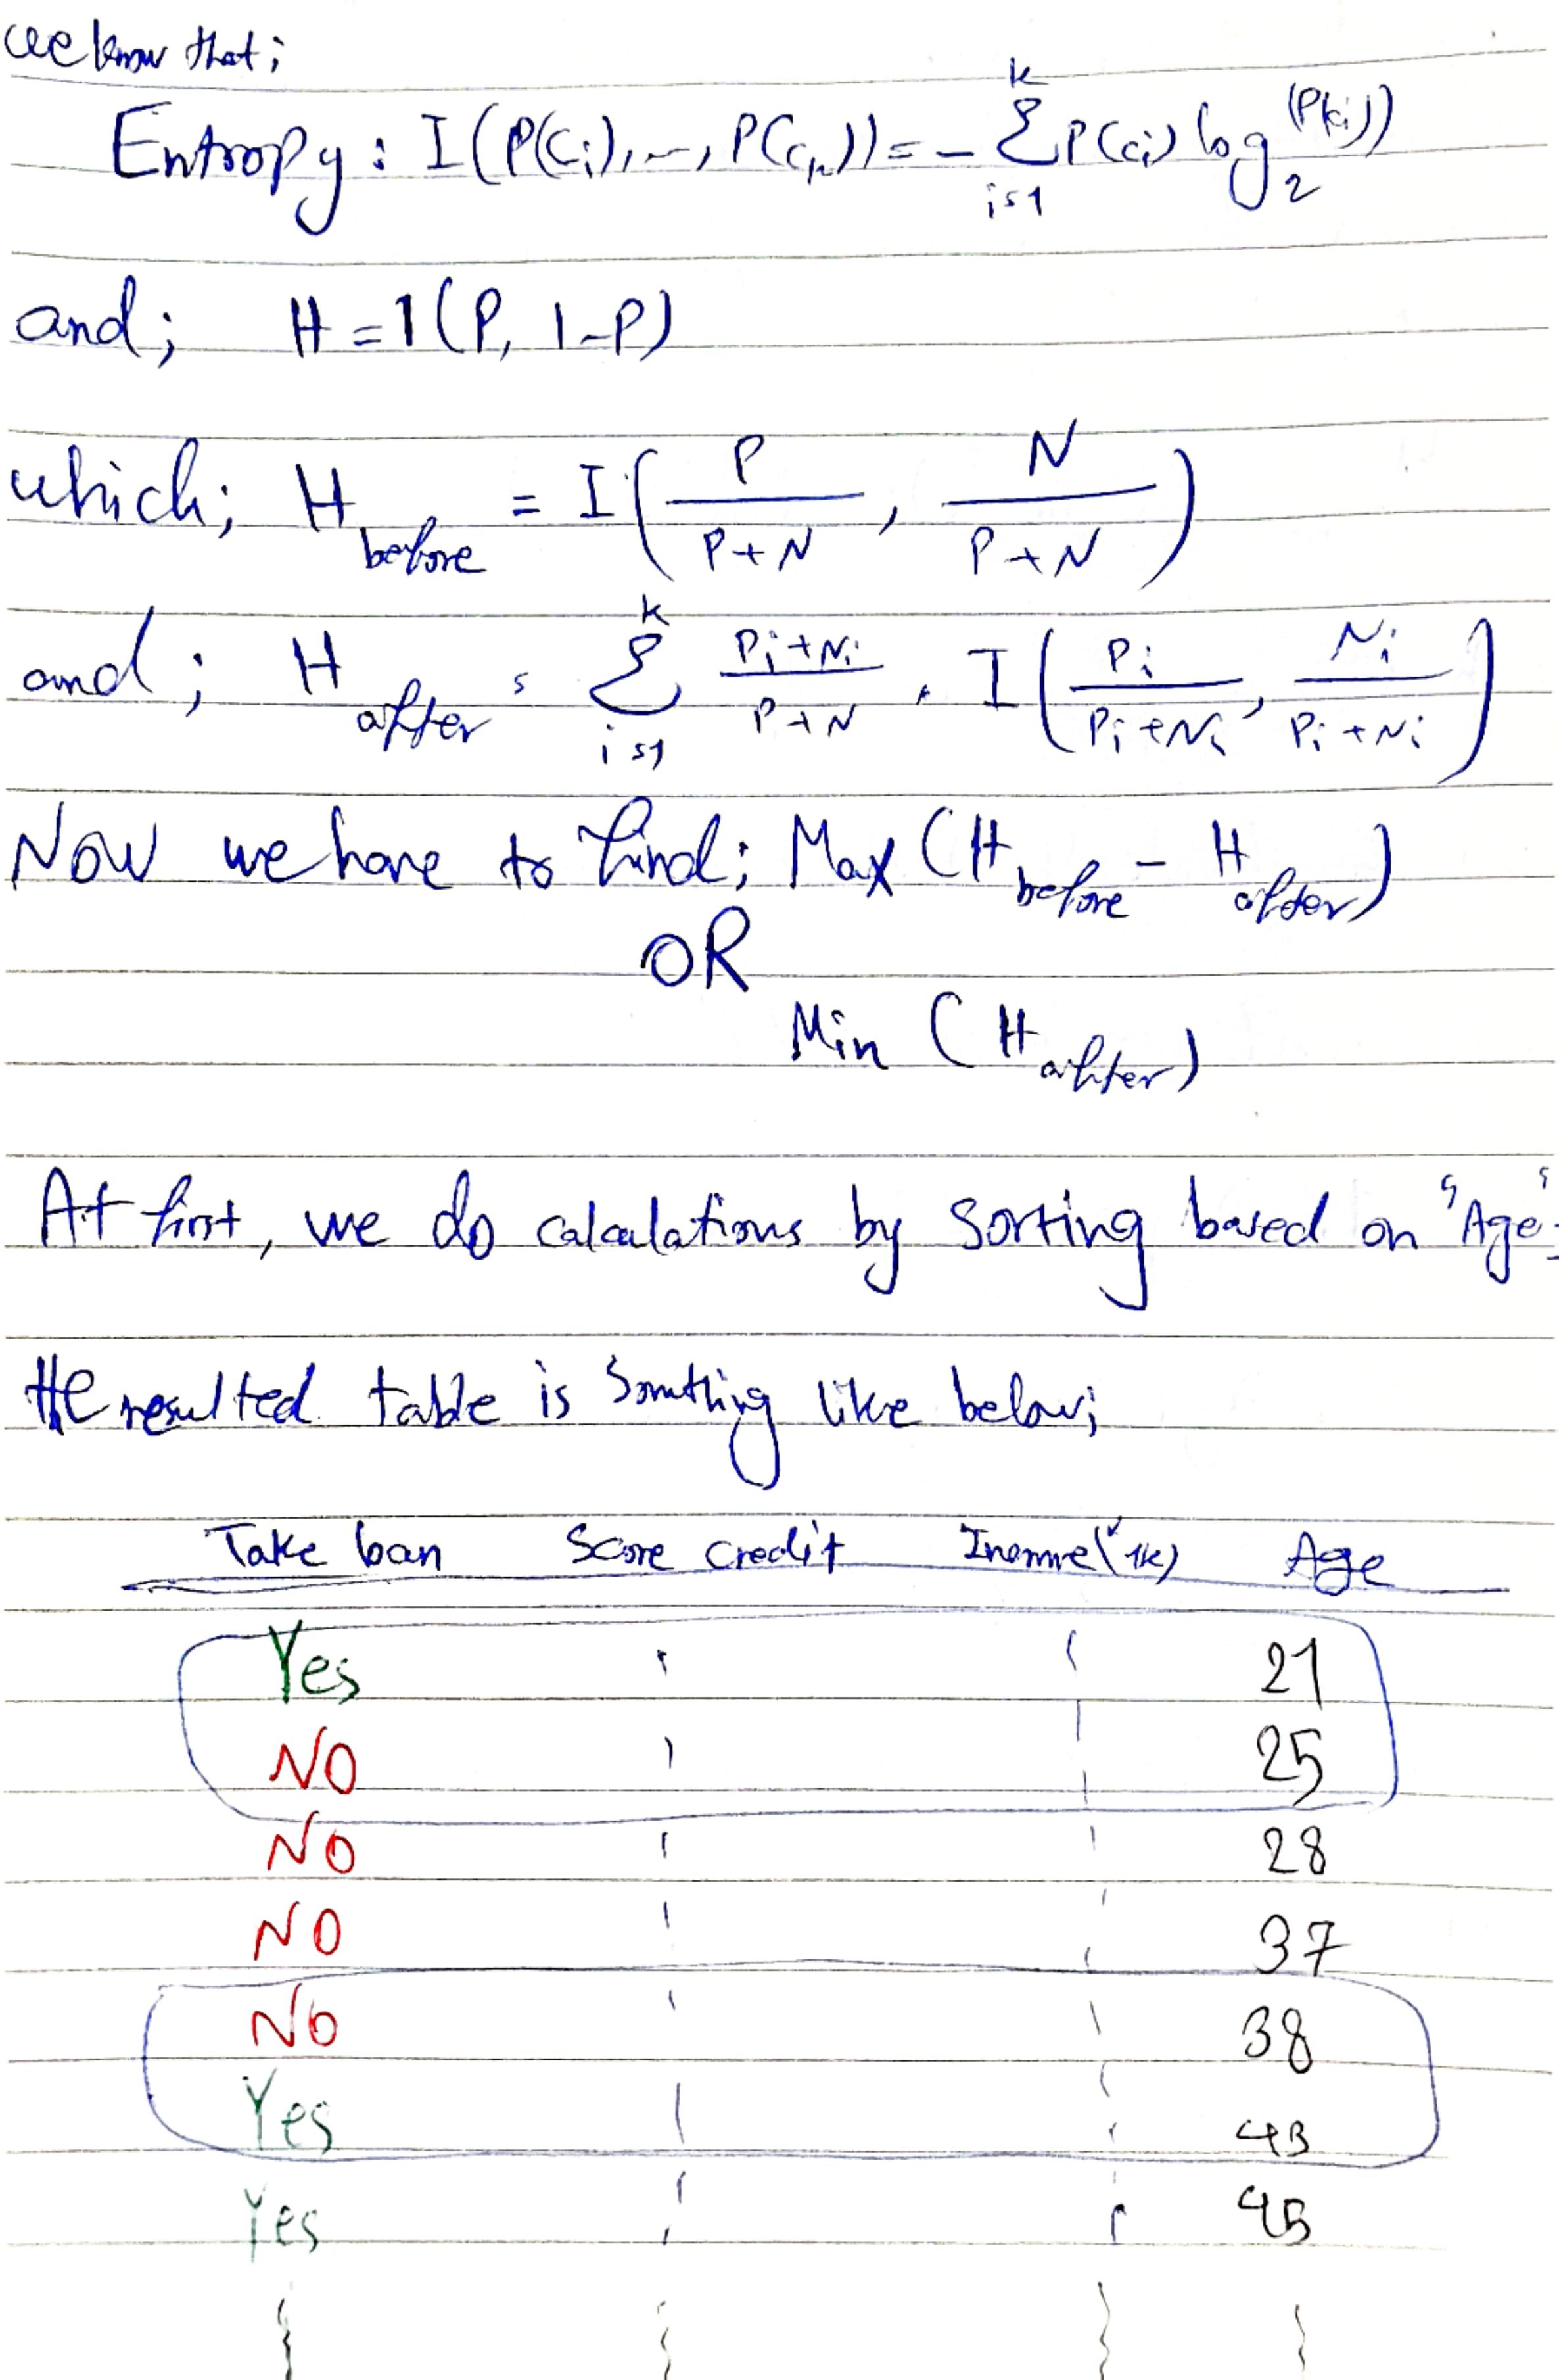
\includegraphics[width=0.84\textwidth]{1.jpg}
	\end{figure}
	\pagebreak
		\begin{figure}[h!]
		\centering
		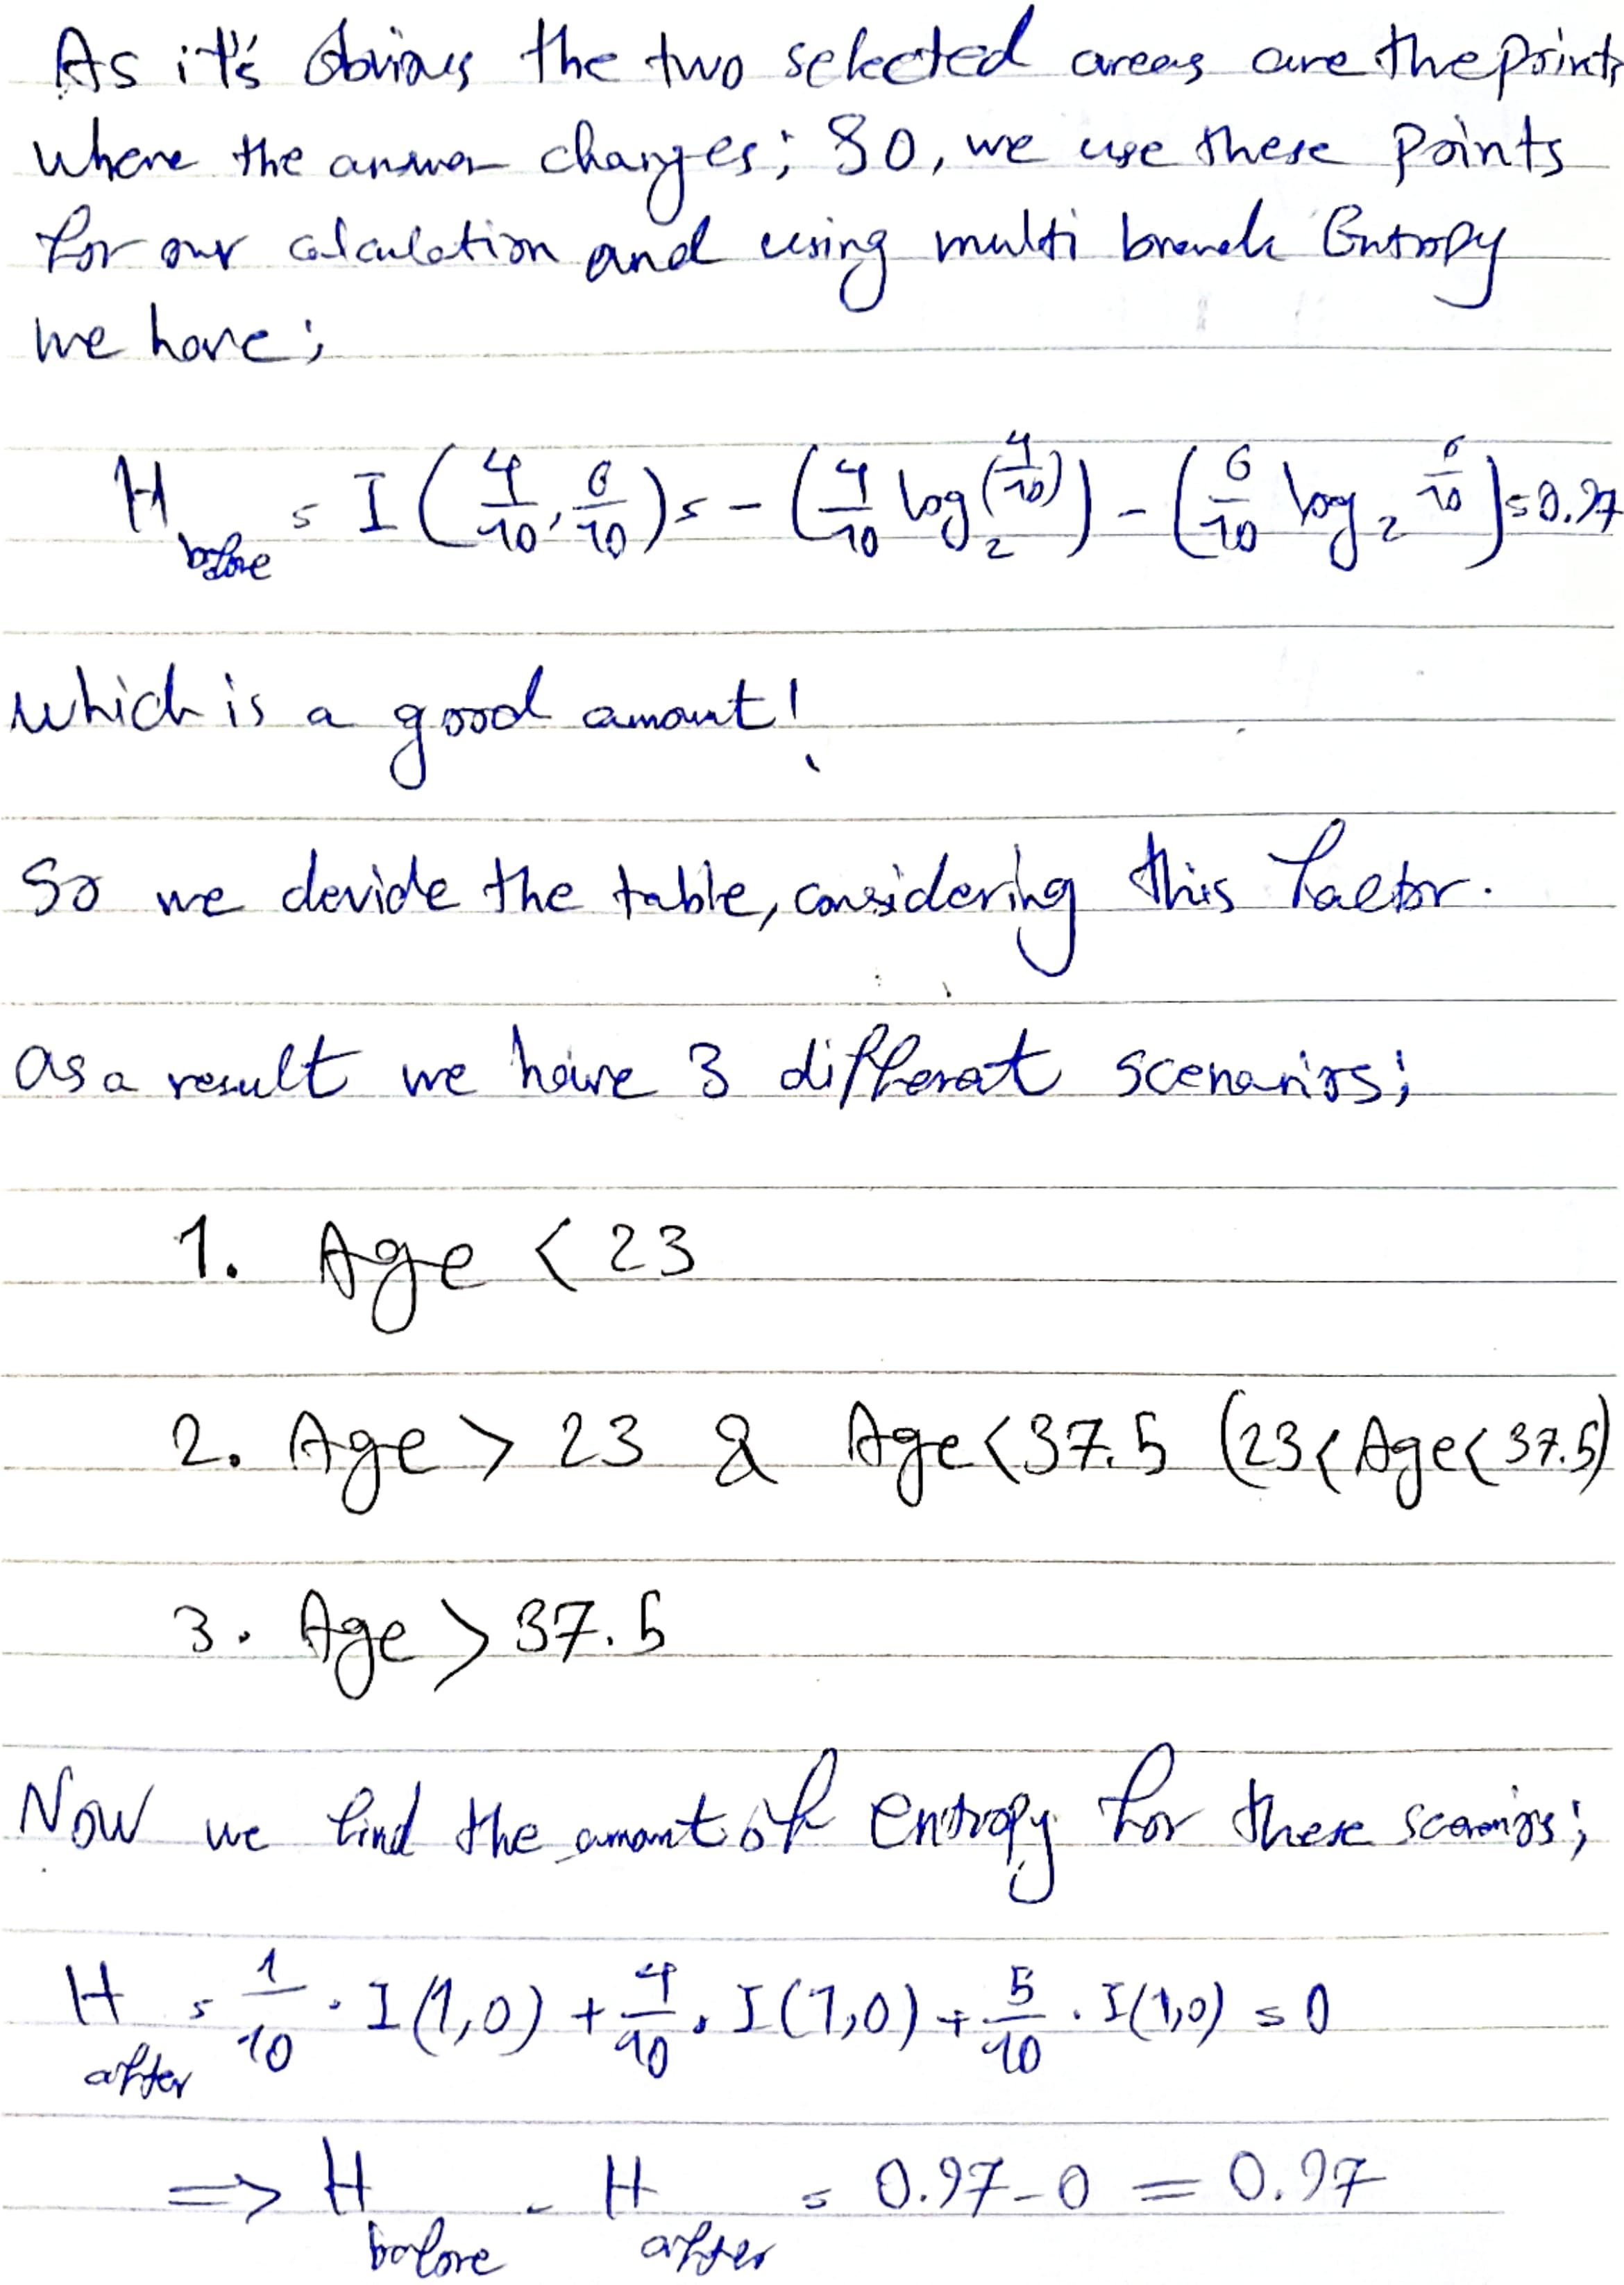
\includegraphics[width=0.84\textwidth]{2.jpg}
	\end{figure}
	\pagebreak
		\begin{figure}[h!]
		\centering
		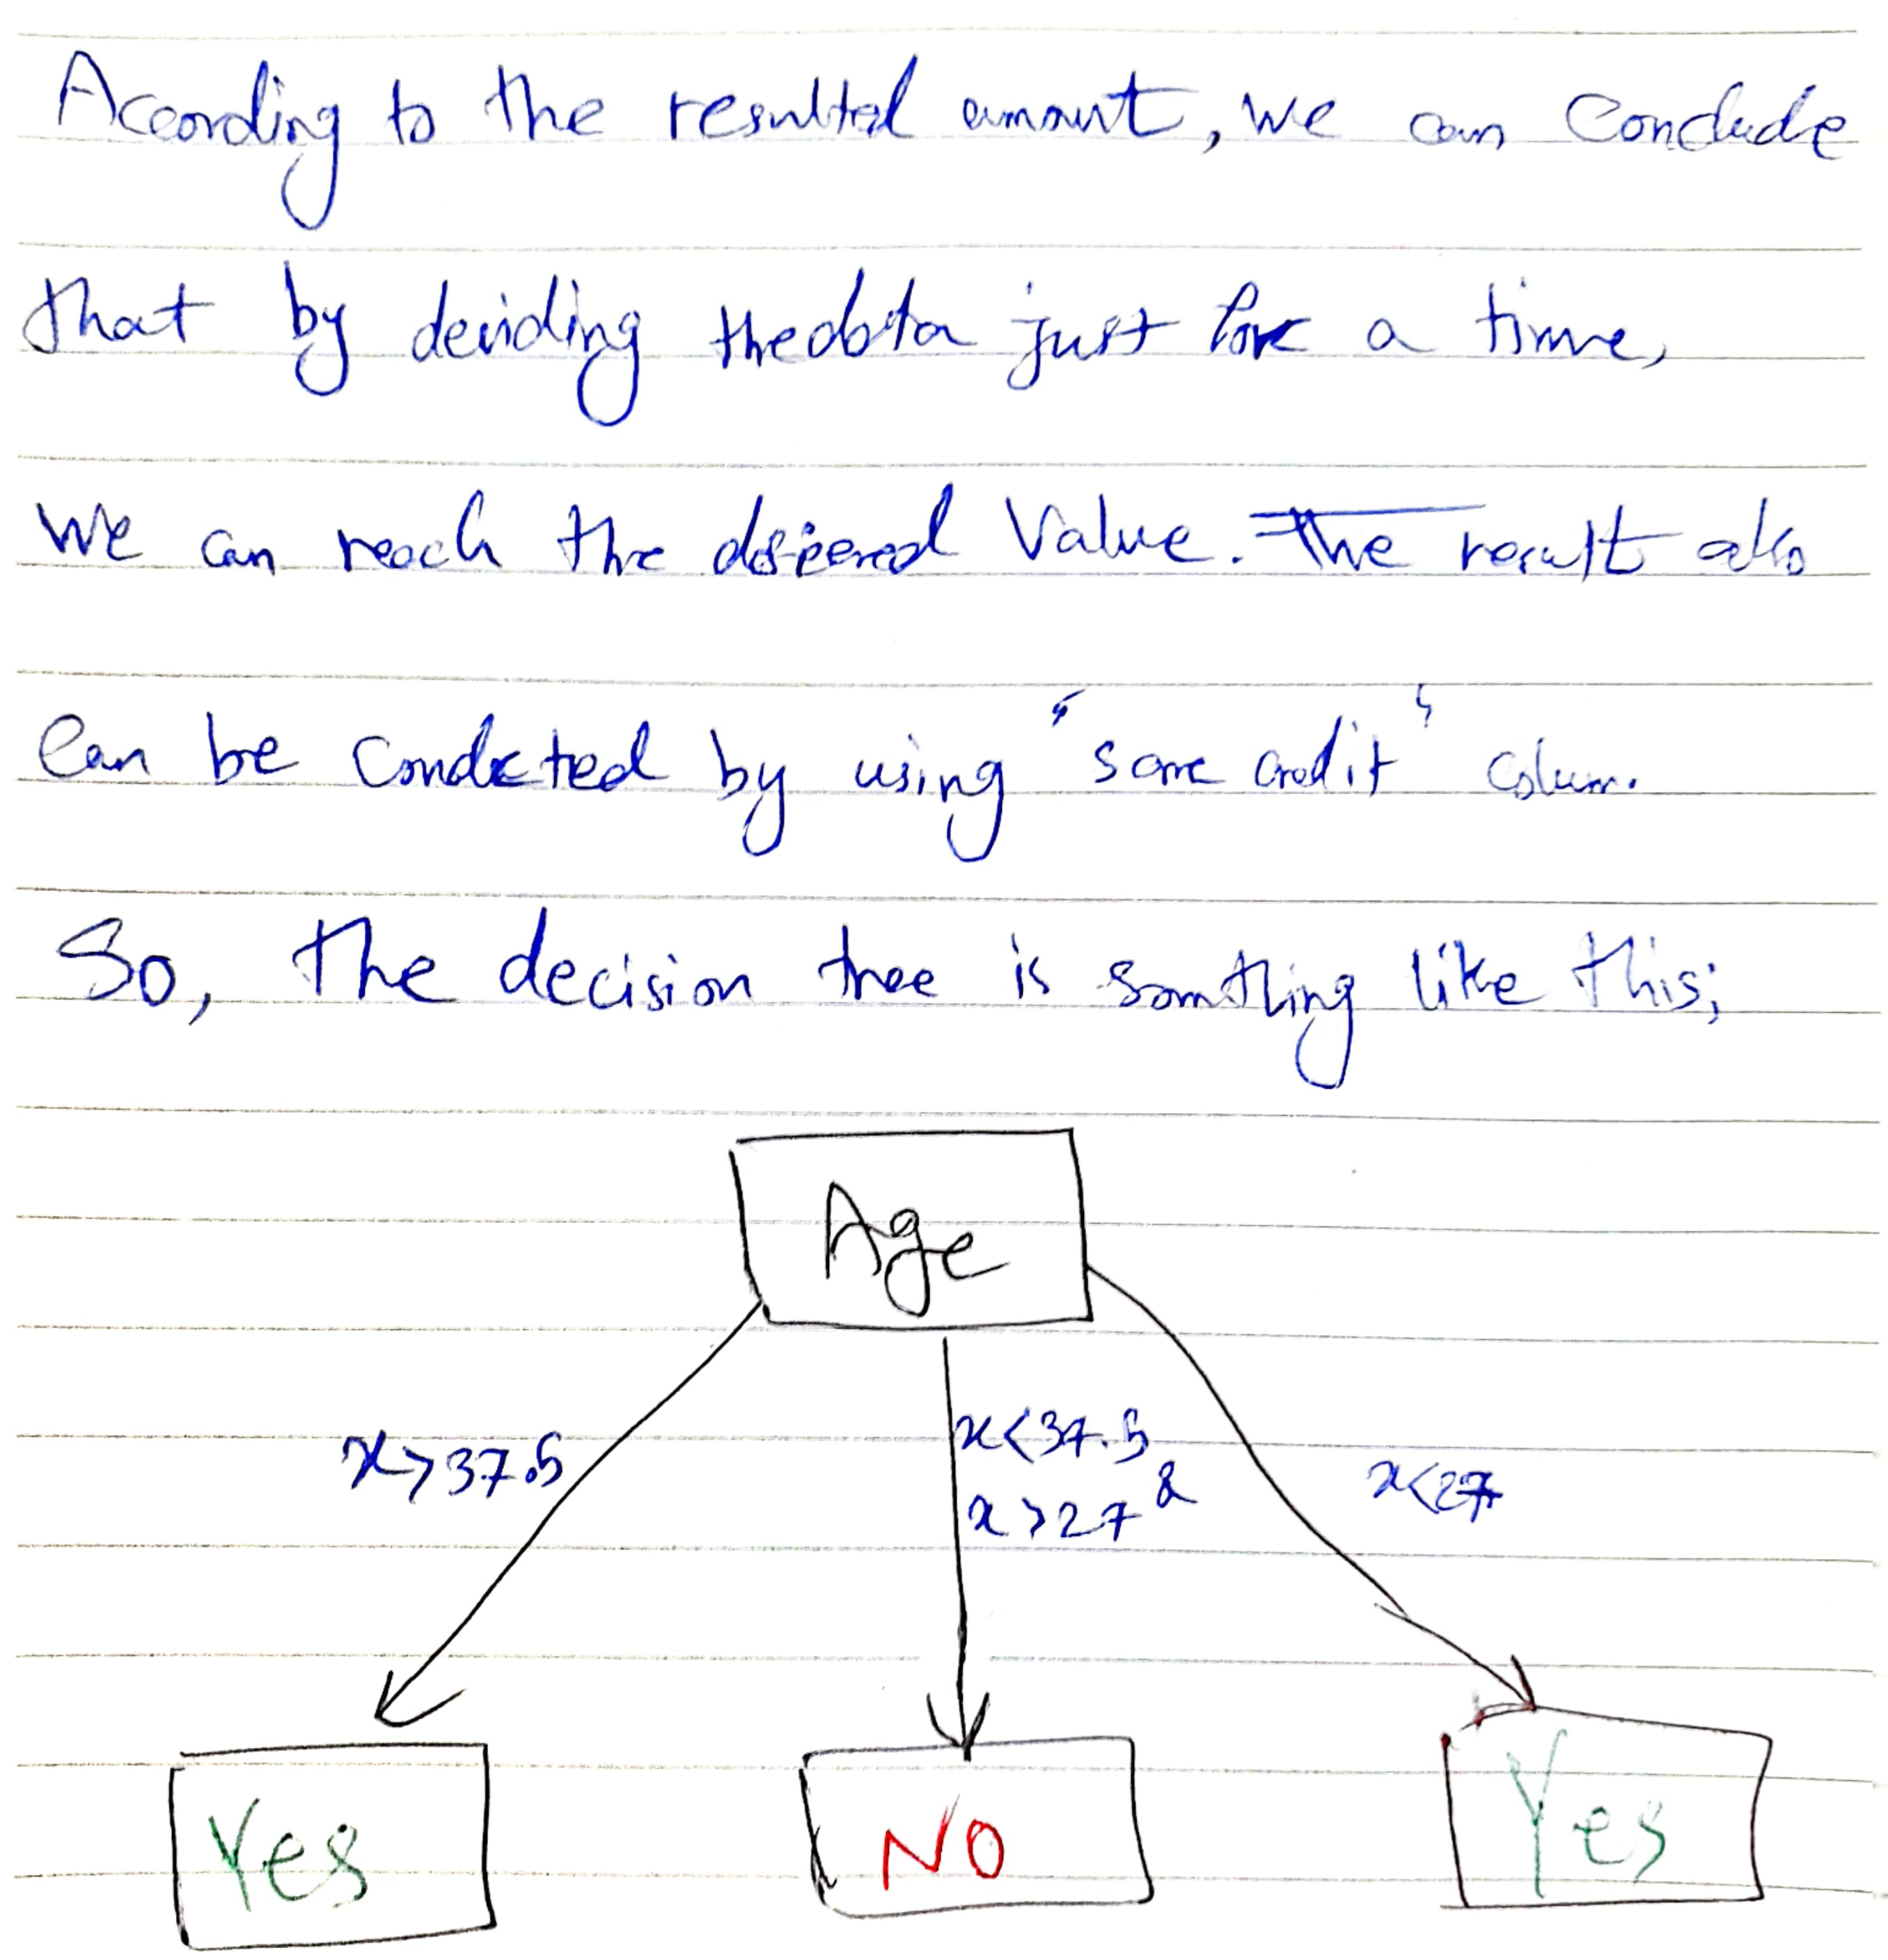
\includegraphics[width=0.84\textwidth]{3.jpg}
	\end{figure}
\end{solution}
\\\noindent\rule{7in}{2.8pt}
\pagebreak
%%%%%%%%%%%%%%%%%%%%%%%%%%%%%%%%%%%%%%%%%%%%%%%%%%%%%%%%%%%%%%%%%%%%%%%%%
\end{document}
 